% Eingangsdaten der Simulation

\section{Modelleingangsdaten}

Grundlage für die Lastflussberechnung durch \edisgo bilden verschiedene Modelleingangsdaten.
Hierzu gehören in erster Linie die mit \simbev erzeugten Lastprofile der Ladevorgänge der \gls{EPKW}, sowie die Erzeugungsprofile erneuerbarer Energieanlagen in einem Netzgebiet.
Weiterhin gehen auch die Lastprofile von Wärmepumpen in die Lastflussberechnung mit ein.

\subsection{Erzeugung der Lastprofile der Ladevorgänge von E-Pkw}

Mit Hilfe des im Rahmen dieser Masterarbeit mitentwickelten Software Tools \simbev können die Fahrtprofile für eine beliebige Anzahl an Fahrzeugen für einen Regionstypen erstellt werden.
Die Fahrtprofile enthalten die gefahrenen Strecken und die Standzeiten am Zielort.
Aus diesen können anschließend anhand des Verbrauchs und der gegebenen Ladeinfrastruktur die Lastprofile der Ladevorgänge abgeleitet werden.\medskip

Die Fahrtprofile werden über einen pro­ba­bi­lis­tischen Ansatz auf Grundlage der Befragung \gls{MID} \cite{ISGH2017} erzeugt.
Dabei erhält jeder simulierte Zeitschritt eine Wahrscheinlichkeit für einen bestimmten Wegezweck eine Fahrt zu beginnen.
Abhängig vom Wegezweck und Regionstyp wird der Fahrt ebenfalls pro­ba­bi­lis­tisch eine Streckenlänge und eine anschließende Standzeit zugeordnet.
Der entstehende Ladebedarf muss anschließend gedeckt werden.
Ob am Zielort ein Ladevorgang stattfindet, hängt vom \gls{SOC} des Fahrzeuges und dem vorhandensein eines Ladepunktes ab.
Ob ein Ladepunkt am Zielort zur Verfügung steht und welche Ladeleistung dieser aufweist, wird mit Hilfe der Wahrscheinlichkeiten aus \autoref{tab:WegezweckProbability2035} bzw. \autoref{tab:WegezweckProbability2050} ermittelt.
Die Bestimmung des vorhandenseins eines Ladepunktes zu Hause und am Arbeitsplatz erfolgt je \gls{EPKW} einmalig und wird anschließend konstant gehalten.
Für alle anderen Wegezwecke, erfolgt die Bestimmung kontinuierlich.
Wurde dem Zielort ein Ladepunkt zugeordnet wird davon ausgegangen, dass der Fahrzeugnutzer einen Ladevorgang erst ab einem bestimmten \gls{SOC} einleitet, da dies einen zusätzlichen Aufwand für den Nutzer bedeutet.
Dabei wird angenommen, dass das Laden des Fahrzeuges am Wohnort und am Arbeitsplatz bereits ab einem \gls{SOC} von \SI{95}{\percent} stattfindet.
Im öffentlichen Raum bedeutet das Anfahren und der Anschluss an einen Ladepunkt einen größeren Aufwand für den Nutzer als im privaten Raum.
Deshalb wird angenommen, dass oberhalb eines \glspl{SOC} von \SI{80}{\percent} keine Ladevorgänge stattfinden.
Es gilt je niedriger der \gls{SOC}, desto wahrscheinlicher ist es, dass die öffentliche Ladeinfrastruktur genutzt wird.
Ab einem \gls{SOC} von \SI{50}{\percent} findet wann immer möglich eine Ladung des Fahrzeugs statt.
Zwischen den beiden Stützwerten erfolgt eine lineare Interpolation, welche in \autoref{fig:soc_charging_prob} visualisiert wurde.

\begin{figure}[H]
    \centering
    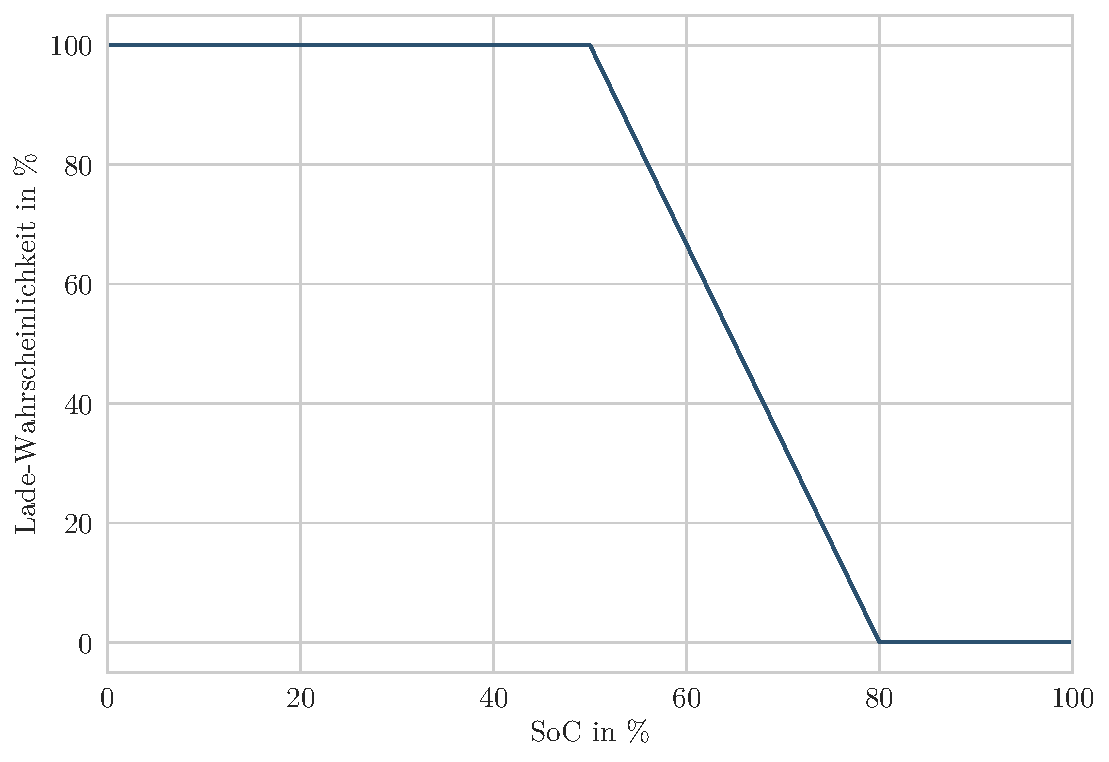
\includegraphics[width=\textwidth]{Bilder/soc_charging_prob}
    \caption{Abhängigkeit der Ladewahrscheinlichkeit vom SoC an öffentlichen Standorten}\label{fig:soc_charging_prob}
\end{figure}

% Schnellladung ab soc 15%